\chapter{ImageNet-to-CIFAR-100 Transfer Teacher and Hierarchy Controls}
\label{app:teacher-transfer-probe}

\section{Purpose}

This appendix documents a first external-teacher probe motivated by Weinshall
et al. \cite{weinshall2018curriculum}. Their curriculum-learning-by-transfer
framework uses a stronger auxiliary model to provide a notion of example
structure before student training. In the present thesis, the analogous
question is whether a stronger external representation can provide a better
\emph{hierarchy source} than the self-derived classifier-weight hierarchies used
in the main coarse-to-fine experiments.

The probe therefore asks two narrower questions:

\begin{enumerate}
    \item can a lightweight ImageNet-initialized ResNet-18 be adapted to
          CIFAR-100 strongly enough to serve as a practical teacher,
    \item if so, does its resulting representation look promising as a source
          for a stronger curriculum hierarchy in later experiments?
\end{enumerate}

This is not yet a curriculum run. It is a teacher-quality probe whose main role
is to decide whether teacher-derived hierarchies are worth testing against the
existing self-derived ones.

\section{Setup}

The run used CIFAR-100 \cite{krizhevsky2009learning} with a ResNet-18
\cite{he2016deep} initialized from torchvision ImageNet weights. Unlike the
main thesis ResNet-18 baseline from Appendix~\ref{app:cifar100-model-size-curriculum},
this probe used a transfer-learning style setup: SGD, learning rate 0.01,
weight decay $5\times 10^{-4}$, augmentation enabled, and a 30-epoch budget.
The hierarchy was exported from validation-split teacher embeddings after the
run finished. The exported artifacts included a readable hierarchy description
and the corresponding distance matrix, which made it possible to analyze the
teacher hierarchy directly rather than treating the run only as a
teacher-accuracy probe.

\section{Training trajectory}

The transfer-initialized teacher converged quickly. Test accuracy reached
0.7730 by epoch 12, 0.7785 by epoch 14, and peaked at 0.7814 at epoch 22. The
final epoch remained essentially unchanged at 0.7810. This trajectory suggests
that the run was already near saturation by 30 epochs, so the probe was not
obviously undertrained.

A useful practical conclusion follows: for the purpose of obtaining a stronger
teacher hierarchy, a short transfer-learning run appears sufficient. The model
already enters the high-0.77 accuracy regime well before epoch 30, which means
that a teacher hierarchy can likely be obtained without the cost of a long
from-scratch CIFAR-100 training schedule.

\section{Comparison with previous CIFAR-100 thesis runs}

Table~\ref{tab:teacher-probe-comparison} compares this teacher probe against the
main thesis CIFAR-100 ResNet-18 results from
Appendix~\ref{app:cifar100-model-size-curriculum}. This comparison does not
isolate a single causal factor, because the protocols differ: the earlier
appendix used an uninitialized ResNet-18 with Adam, no scheduler, and a
100-epoch budget, while the present run used ImageNet initialization, SGD,
augmentation, and only 30 epochs. Even with that caveat, the magnitude of the
improvement is large enough to be informative.

\begin{table}[h]
\centering
\small
\begin{tabular}{lrrr}
\hline
Condition & Best test acc. & Delta vs old baseline & Delta vs old best curriculum \\
\hline
Old ResNet-18 baseline (Appendix~\ref{app:cifar100-model-size-curriculum}) & 0.6876 & -- & -- \\
Old ResNet-18 best curriculum (20 epochs) & 0.6937 & +0.61 pp & -- \\
Transfer-initialized teacher probe & 0.7814 & +9.38 pp & +8.77 pp \\
\hline
\end{tabular}
\caption{Teacher probe against previous thesis CIFAR-100 ResNet-18 results.}
\label{tab:teacher-probe-comparison}
\end{table}

Two conclusions matter here.

First, the transfer-initialized run is substantially stronger than the previous
thesis ResNet-18 regime. Even after allowing for protocol changes, the gap is
large enough that the teacher's representation should be treated as materially
stronger than the self-derived hierarchies produced by the weaker thesis
baselines.

Second, the result weakens any interpretation that the earlier thesis ResNet-18
numbers represented the practical ceiling for CIFAR-100 in this codebase. The
teacher probe shows that a stronger operating point is reachable with moderate
cost, which makes external-teacher hierarchies a credible next step rather than
just a speculative extension.

\section{Returned hierarchy analysis}

The exported hierarchy is qualitatively much cleaner than the weak self-derived
CIFAR-100 hierarchies discussed in Appendix~\ref{app:roughness-followup-curriculum}.
Its top level has only three broad groups, which are still somewhat mixed, but
already more interpretable than the previous classifier-weight trees from weak
CNNs:

\begin{itemize}
    \item a large natural-object cluster dominated by fruits, flowers, insects,
          reptiles, and many mammals,
    \item a mixed aquatic/human/household cluster containing fish and sea
          mammals together with people and indoor objects,
    \item a vehicles-and-scenes cluster containing transport classes, built
          structures, landscapes, and trees.
\end{itemize}

The top level is therefore still too coarse to be treated as a human-semantic
ontology. However, the second level is the more important diagnostic for the
curriculum, and there the structure becomes much stronger. The recovered
23-cluster partition contains many coherent groups, for example:

\begin{itemize}
    \item fruits and flowers: \texttt{apple, rose, sunflower, sweet\_pepper,
          orange, orchid, pear, tulip, poppy},
    \item aquatic animals: \texttt{aquarium\_fish, shark, trout, dolphin,
          whale},
    \item people: \texttt{baby, girl, woman, boy, man},
    \item large mammals: \texttt{bear, beaver, seal, lion, skunk, camel,
          cattle, chimpanzee, otter, porcupine, elephant},
    \item furniture: \texttt{couch, chair, bed, table},
    \item insects and nearby small creatures: \texttt{cockroach, bee,
          beetle},
    \item road vehicles: \texttt{streetcar, train, pickup\_truck, bus},
    \item natural scenes: \texttt{mountain, plain, sea, cloud},
    \item trees: \texttt{willow\_tree, forest, oak\_tree, palm\_tree,
          pine\_tree, maple\_tree}.
\end{itemize}

This second-level structure is exactly the kind of evidence that was missing
from the weaker self-derived hierarchies. In the earlier appendix, the learned
clusters were often visually or semantically mixed enough to explain why the
curriculum gains were limited or unstable. At the same time, the teacher-derived
hierarchy should not be judged only as a human taxonomy. Some groupings that
look semantically loose to a human reader may still be meaningful for a CNN
because they reflect image-distribution properties such as shape, texture,
background, object scale, or typical viewpoint. Conversely, a human-semantic
category such as ``vehicles'' can group classes that look quite different in
CIFAR-100 images. The hierarchy is therefore best interpreted as a
representation-induced class partition, not as an ontology. Under that criterion,
its overall organization is markedly more plausible than the weaker
self-derived alternatives. That makes it a credible candidate for testing
whether hierarchy quality, rather than output-space curriculum as such, was the
limiting factor in the earlier experiments.

A second practical observation is that the teacher hierarchy is also much deeper
than the official CIFAR-100 superclass taxonomy. Instead of one manually defined
20-way superclass layer, it offers a learned progression from 3 broad groups to
23 intermediate groups and finally the singleton fine classes. This is useful
for follow-up experiments because it enables both a direct coarse-to-fine test
and a more controlled anti-curriculum test on the same learned structure.

\section{Why this matters for the curriculum experiments}

The main vision-track results in this thesis showed that the current
coarse-to-fine curriculum can improve peak accuracy conditionally, but usually
pays an AUC penalty and does not reproduce the strong early-speed benefits seen
in teacher-ranked instance curricula such as Weinshall et al.
\cite{weinshall2018curriculum}. One plausible explanation was that the
hierarchy source itself was too weak or too self-referential: the main thesis
hierarchies were derived from the target training setup rather than from a much
stronger external model.

The present teacher probe supports that hypothesis well enough to justify a
follow-up experiment suite. A 0.78-level transfer teacher is plausibly strong
enough to produce a cleaner class-similarity structure than the weaker
classifier-weight hierarchies derived from the original CNN baselines. This does
not guarantee that the curriculum will become stronger, but it makes the next
comparison well motivated:

\begin{enumerate}
    \item self-derived hierarchy,
    \item external teacher-embedding hierarchy,
    \item random hierarchy control,
    \item anti-curriculum control.
\end{enumerate}

This comparison is especially relevant in light of Weinshall et al., because it
would test whether transferring \emph{structure} from a stronger model helps the
output-space curriculum regime in the same general spirit that transferred
example difficulty helped their instance-based curriculum.

\section{Teacher-hierarchy curriculum follow-up}

The follow-up experiment used the strongest cheap student setup from the earlier
CIFAR-100 appendices: \texttt{cnn\_w0.5}, Adam with learning rate 0.001, batch
size 128, a 100-epoch budget, and a fixed 20-epoch coarse-to-fine curriculum.
The comparison used three training seeds (42, 43, 44). For each seed, the
baseline, the self-derived hierarchy, and the random hierarchy controls were
reused from the first completed suite. The teacher-dependent runs were then
rerun with a corrected transfer teacher: a ResNet-18 initialized from ImageNet,
trained for 30 epochs with SGD and learning rate 0.01. This corrected teacher
reached 77.65\% best CIFAR-100 test accuracy, close to the earlier 78.14\%
teacher probe and substantially above the first bootstrap teacher, which had
reached only 72.40\% with learning rate 0.1.

The methods compared below are:

\begin{itemize}
    \item \textbf{Baseline}: ordinary fine-label training.
    \item \textbf{Random}: random permutations of the learned hierarchy shape;
          this preserves the number of levels and cluster sizes but destroys
          semantic grouping.
    \item \textbf{Anti}: a reverse-order hierarchy control using the corrected
          teacher hierarchy. It reverses the order of the non-singleton hierarchy
          levels, but still ends with ordinary fine-label training.
    \item \textbf{Self/regular}: the standard classifier-weight hierarchy used
          in the previous CIFAR-100 \texttt{cnn\_w0.5} experiments.
    \item \textbf{Teacher}: the corrected teacher-embedding hierarchy from the
          77.65\% transfer teacher.
\end{itemize}

This setup intentionally separates two questions. The random control asks
whether merely bundling labels---even incorrectly---can help. The anti-curriculum
asks whether a structured hierarchy still helps when the temporal order is wrong.
The self and teacher rows then test whether using a semantically or
representation-aligned hierarchy improves beyond these weaker controls.

\section{What the anti-curriculum means in this implementation}

The word ``anti-curriculum'' needs a precise definition here, because it can be
misread as training on intentionally wrong labels. That is not what is done in
this thesis. The anti-curriculum uses the same learned hierarchy as the teacher
condition and the same marginalised coarse-label loss. The only change is the
order in which the non-singleton hierarchy levels are visited.

For a typical teacher hierarchy, the effective curriculum levels are roughly:

\begin{center}
\begin{tabular}{lll}
\hline
Regime & Stage order before fine-tuning & Meaning \\
\hline
Easy-to-hard & 3--5 clusters $\rightarrow$ 23--24 clusters & coarse to less coarse \\
Anti / reverse & 23--24 clusters $\rightarrow$ 3--5 clusters & less coarse to coarse \\
\hline
\end{tabular}
\end{center}

Both regimes then finish with the same singleton fine-label stage. Thus the
anti-curriculum is better described as a \emph{reverse-order hierarchy control}:
it starts from the finest non-singleton grouping, moves to a coarser grouping,
and only then switches to the ordinary 100-class objective. It is not a pure
negative control and it is not equivalent to random labels.

The loss also matters. The model always has 100 logits. During a coarse stage,
an image with fine label $y$ is assigned to the current cluster $C(y)$, and the
loss rewards probability mass anywhere in that cluster:

\[
    \mathcal{L}_{\mathrm{coarse}}(x,y)
    = -\log \sum_{c \in C(y)} p_\theta(c \mid x).
\]

If the current cluster is small, this objective is already close to the final
fine-label objective. For example, a 24-cluster level on CIFAR-100 has an average
cluster size of about four classes. A 3-cluster level has an average cluster
size above thirty classes. Therefore the anti-curriculum can show noticeably
higher 100-way test accuracy early in training: it is not secretly using fine
labels, but its first stage is a much finer proxy task than the first stage of
the easy-to-hard curriculum.

This distinction explains the otherwise surprising early behaviour. In the
corrected teacher run, the easy-to-hard teacher curriculum starts around 3--5
clusters and reaches about 2.1\% test accuracy after one epoch, while the
anti-curriculum starts around 23--24 clusters and reaches about 5.7\%. Both are
far below the fine-label baseline at the same epoch, but anti is higher because
it receives a more fine-grained coarse signal. Later in the coarse phase, anti
moves backwards to 3--5 clusters, so its fine-label accuracy stagnates before the
final fine-label stage begins.

This is why the anti result should be interpreted cautiously. If it performs
well, that does not mean that reversing the curriculum is beneficial in the
usual pedagogical sense. It means that structured label bundles can remain
useful even when the temporal order is wrong, and that starting with a
near-fine-grained coarse task can already provide a substantial warm-up.

\section{Aggregate result: random and anti-curricula are above baseline}

Table~\ref{tab:teacher-hierarchy-controls-aggregate} summarizes the merged
comparison. The surprising result is that both random coarsening and
anti-curriculum are above the baseline in best accuracy. Random hierarchies give
an average gain of +0.97 percentage points, and the best random hierarchy among
three random seeds per training seed gives +1.20 points. The anti-curriculum is
stronger still at +2.06 points. The regular self hierarchy and the corrected
teacher hierarchy remain higher, at +2.39 and +2.31 points respectively, but the
random and anti controls are not failures. In this table, AUC refers to the
normalized test-accuracy trajectory over epochs.

\begin{table}[h]
\centering
\small
\begin{tabular}{lrrrl}
\hline
Method & Best acc. & Best gain & AUC gain & Interpretation \\
\hline
Baseline & 35.38 & -- & -- & fine-label reference \\
Random hierarchy mean & 36.35 & +0.97 & -5.82 & random label bundling helps \\
Teacher anti-curriculum & 37.43 & +2.06 & -3.40 & wrong order, structured groups \\
Self/regular hierarchy & 37.76 & +2.39 & -4.76 & previous learned hierarchy \\
Teacher hierarchy & 37.69 & +2.31 & -3.52 & corrected transfer teacher \\
\hline
\end{tabular}
\caption{CIFAR-100 \texttt{cnn\_w0.5} hierarchy-control comparison. Values are
means over seeds 42, 43, and 44. Gains are percentage points relative to the
matching baseline. AUC gain is the change in normalized test-accuracy trajectory
area. The teacher row uses the corrected 77.65\% transfer teacher.}
\label{tab:teacher-hierarchy-controls-aggregate}
\end{table}

Figure~\ref{fig:teacher-hierarchy-best-gain} shows the same result graphically.
The main pattern is monotone in a useful but imperfect way: random coarsening is
better than no curriculum, anti-curriculum is better than random, and the two
structured easy-to-hard curricula are best on average. The teacher hierarchy is
not meaningfully better than the self-derived hierarchy in peak accuracy, but it
is clearly above random.

\begin{figure}[h]
    \centering
    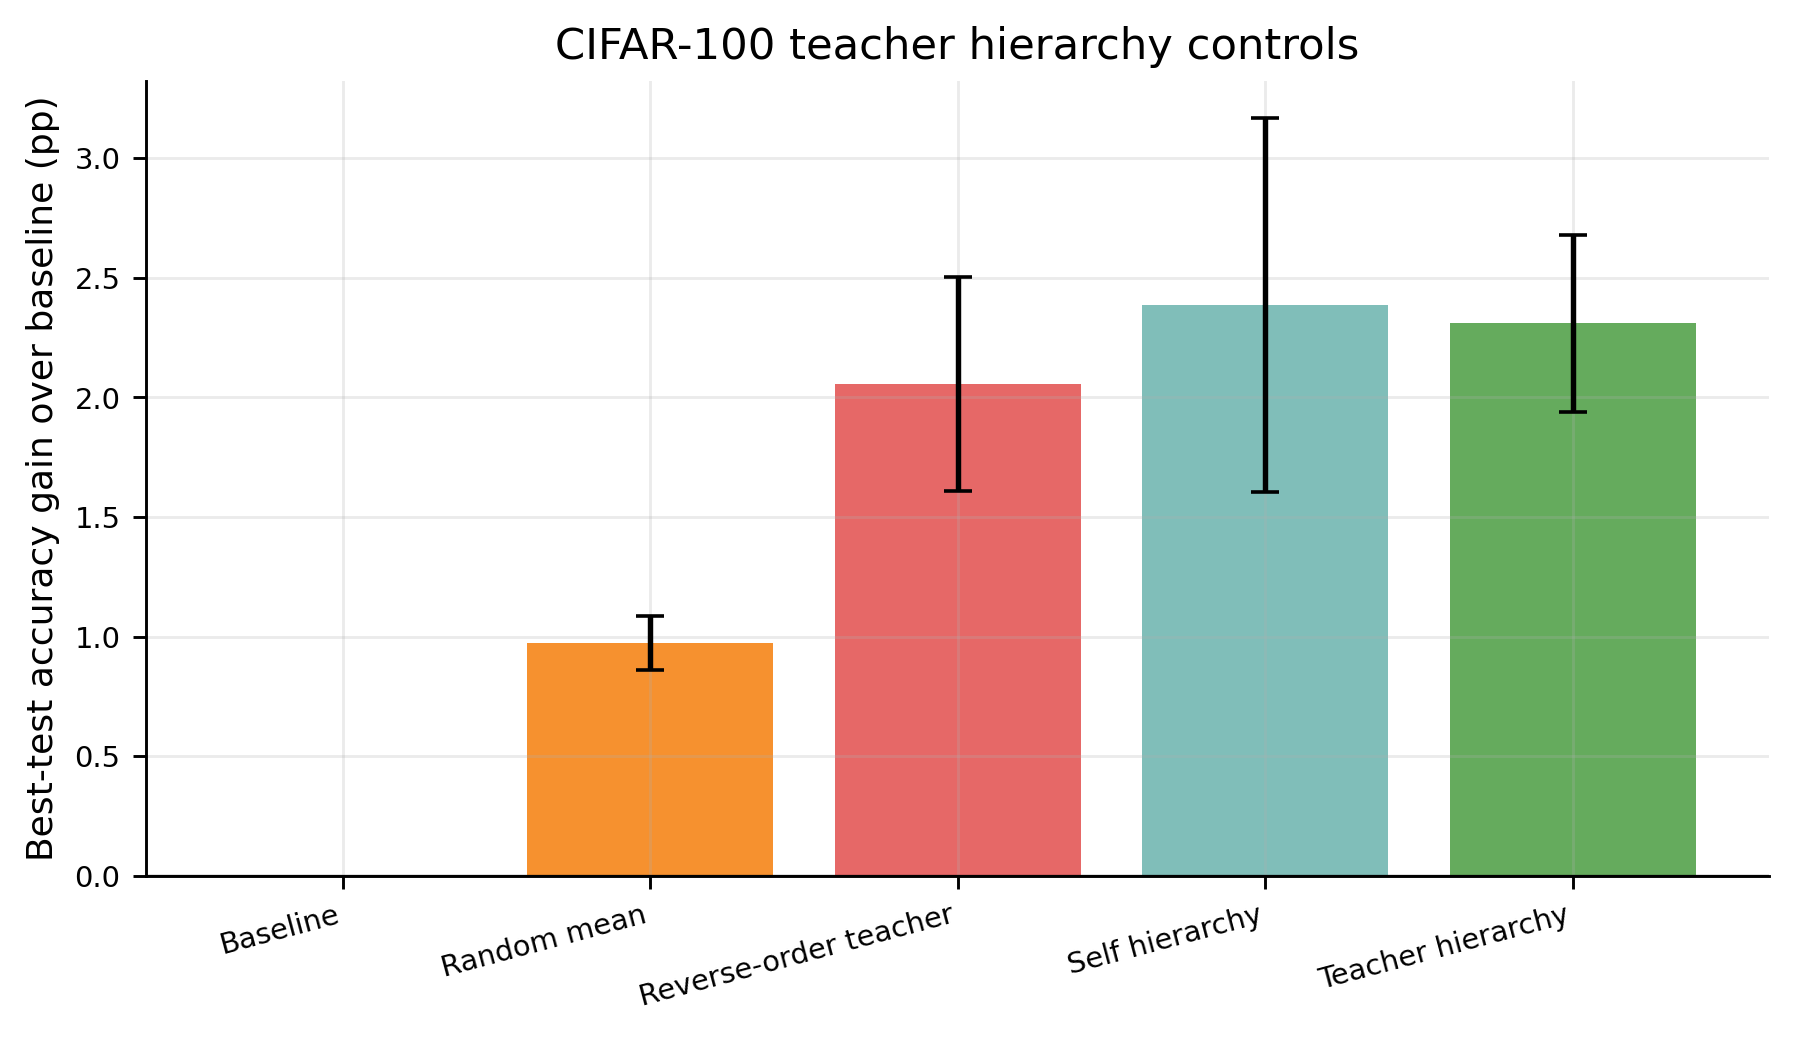
\includegraphics[width=0.86\textwidth]{figures/teacher_hierarchy_best_gain_bar_lr001.png}
    \caption{Best test-accuracy gain over the matching baseline. Random label
    bundling already improves peak accuracy, but structured hierarchies improve
    more. Error bars show standard deviation over three training seeds.}
    \label{fig:teacher-hierarchy-best-gain}
\end{figure}

\section{Per-seed behavior and the random-control surprise}

Table~\ref{tab:teacher-hierarchy-controls-seeds} gives the seed-level best
accuracy values. The random mean beats the baseline for all three seeds, and all
nine individual random hierarchy runs were also above their matching baseline.
This is worth emphasizing because it means the curriculum benefit cannot be
interpreted only as evidence of semantic hierarchy quality. Some of the gain is
created by the training protocol itself: the student spends the first stage
solving a coarser problem, even if the coarse classes are arbitrary.

\begin{table}[h]
\centering
\small
\begin{tabular}{rrrrrrr}
\hline
Seed & Baseline & Random mean & Anti & Self/regular & Teacher & Teacher--random \\
\hline
42 & 35.53 & 36.41 & 38.10 & 37.15 & 37.48 & +1.07 \\
43 & 35.37 & 36.47 & 37.21 & 38.55 & 38.06 & +1.59 \\
44 & 35.23 & 36.16 & 36.99 & 37.59 & 37.52 & +1.36 \\
\hline
Mean & 35.38 & 36.35 & 37.43 & 37.76 & 37.69 & +1.34 \\
\hline
\end{tabular}
\caption{Per-seed best test accuracy for the hierarchy-control follow-up.
Values are percentages. The teacher--random column is the corrected teacher
hierarchy's advantage over the random-hierarchy mean in percentage points.}
\label{tab:teacher-hierarchy-controls-seeds}
\end{table}

Figure~\ref{fig:teacher-hierarchy-seed-gains} makes the same point more clearly.
The gray dots are the individual random hierarchies. Their consistent positive
position shows that random bundling is a real effect in this setup. However, the
orange random mean remains below the anti, self, and teacher curves. Thus the
right interpretation is not that random grouping is as good as curriculum
structure. Rather, random grouping reveals a baseline regularization or
optimization benefit from reducing the effective label space, while meaningful
structure adds an additional benefit on top.

\begin{figure}[h]
    \centering
    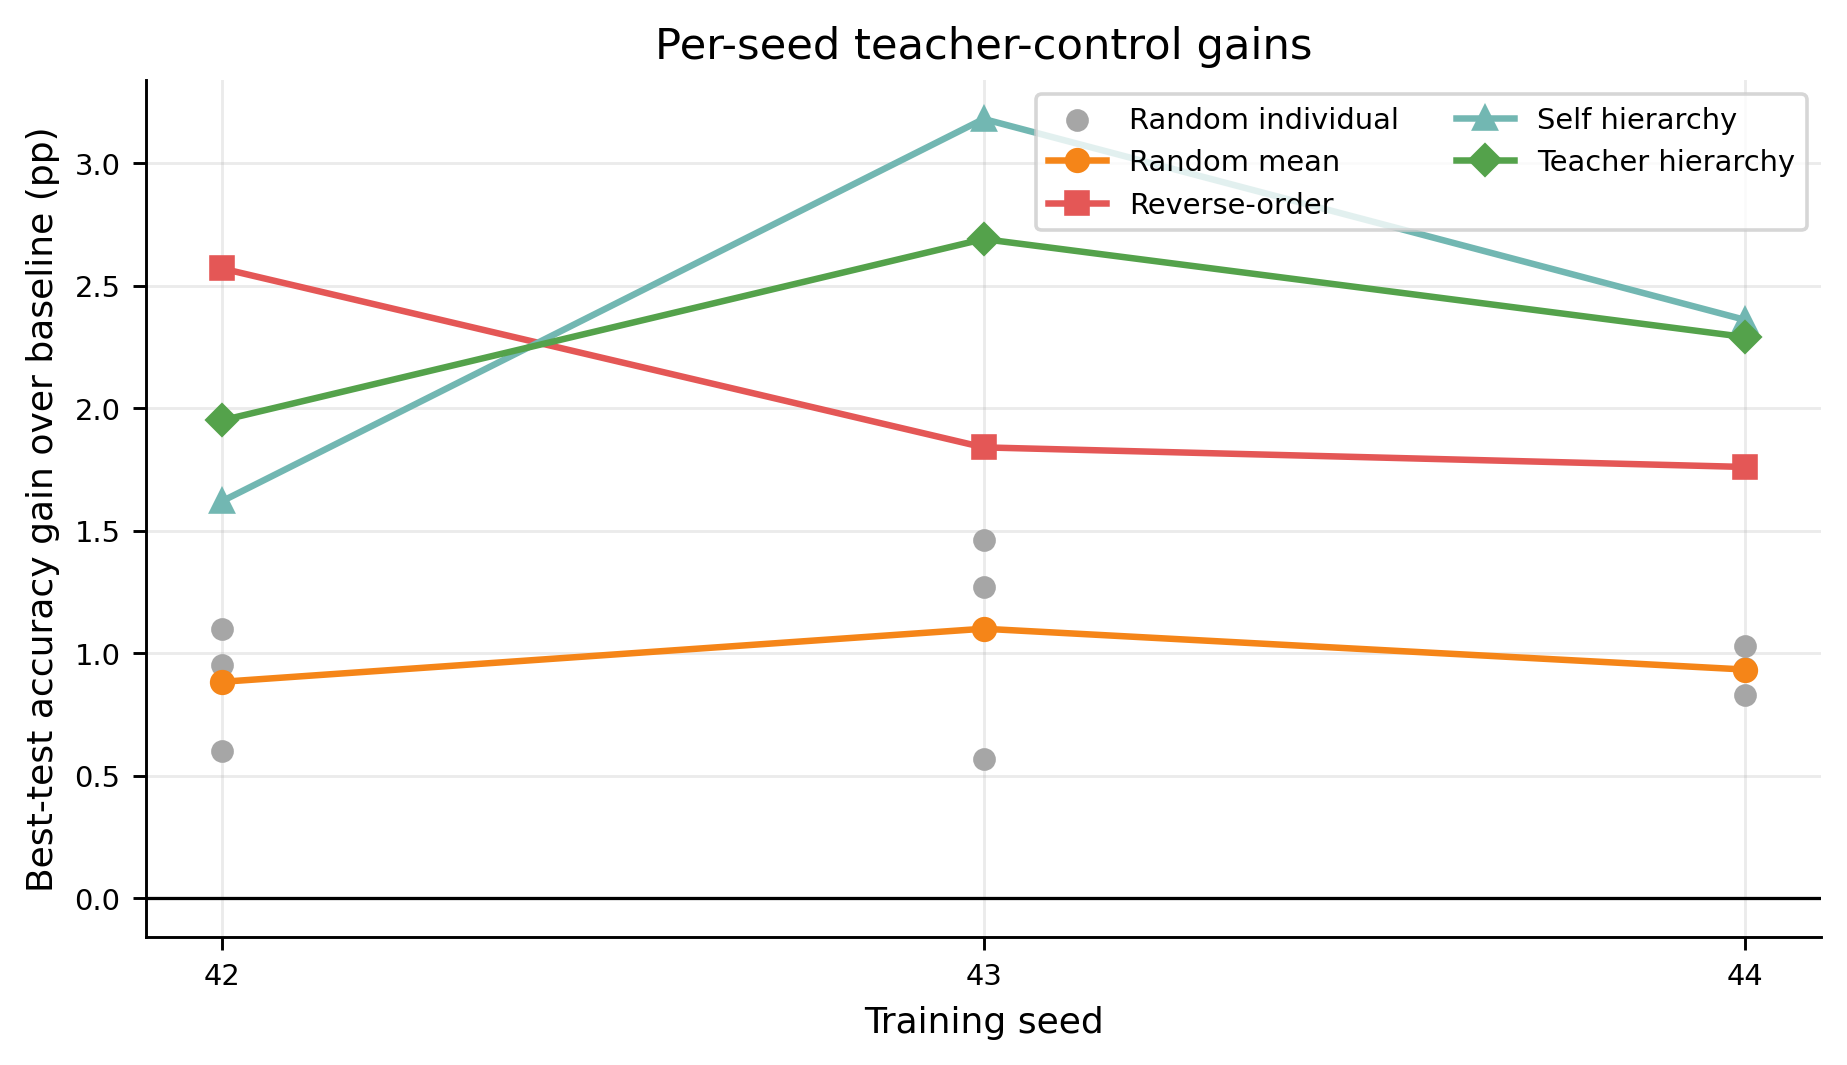
\includegraphics[width=0.90\textwidth]{figures/teacher_hierarchy_seed_gains_lr001.png}
    \caption{Per-seed best-accuracy gains. Gray dots are individual random
    hierarchies; the orange line is their per-seed mean. Random coarsening is
    consistently above baseline, but structured curricula generally sit higher.}
    \label{fig:teacher-hierarchy-seed-gains}
\end{figure}

The anti-curriculum result is slightly different from the random result. Anti is
not random: it still uses the teacher's structured clusters, only in the wrong
order. Its gain therefore suggests that the hierarchy's grouping information can
remain useful even when the easy-to-hard temporal direction is disrupted. At the
same time, anti remains below the best structured easy-to-hard variants on
average, so direction is not irrelevant.

\section{Learning curves: coarse labels hurt early fine accuracy but recover}

Figure~\ref{fig:teacher-hierarchy-learning-curves} plots mean test accuracy
trajectories. The dashed line marks the end of the 20-epoch coarse phase. The
most visible phenomenon is the large early fine-label accuracy deficit for all
curriculum variants. This is expected: during the coarse phase, the model is not
being optimized directly for the final 100-way fine-label objective.

The surprising part happens after the switch. Even random hierarchies recover
above the baseline peak region, although less strongly than the structured
hierarchies. This supports a two-component explanation:

\begin{enumerate}
    \item \textbf{Coarsening effect}: any early coarse-label stage can act as a
          regularizer or optimization warm-up, reducing the effective class
          granularity and changing the early representation learned by the CNN.
    \item \textbf{Structure effect}: meaningful class groupings improve this
          warm-up relative to arbitrary groupings, producing higher peaks for
          self-derived and teacher-derived hierarchies.
\end{enumerate}

\begin{figure}[h]
    \centering
    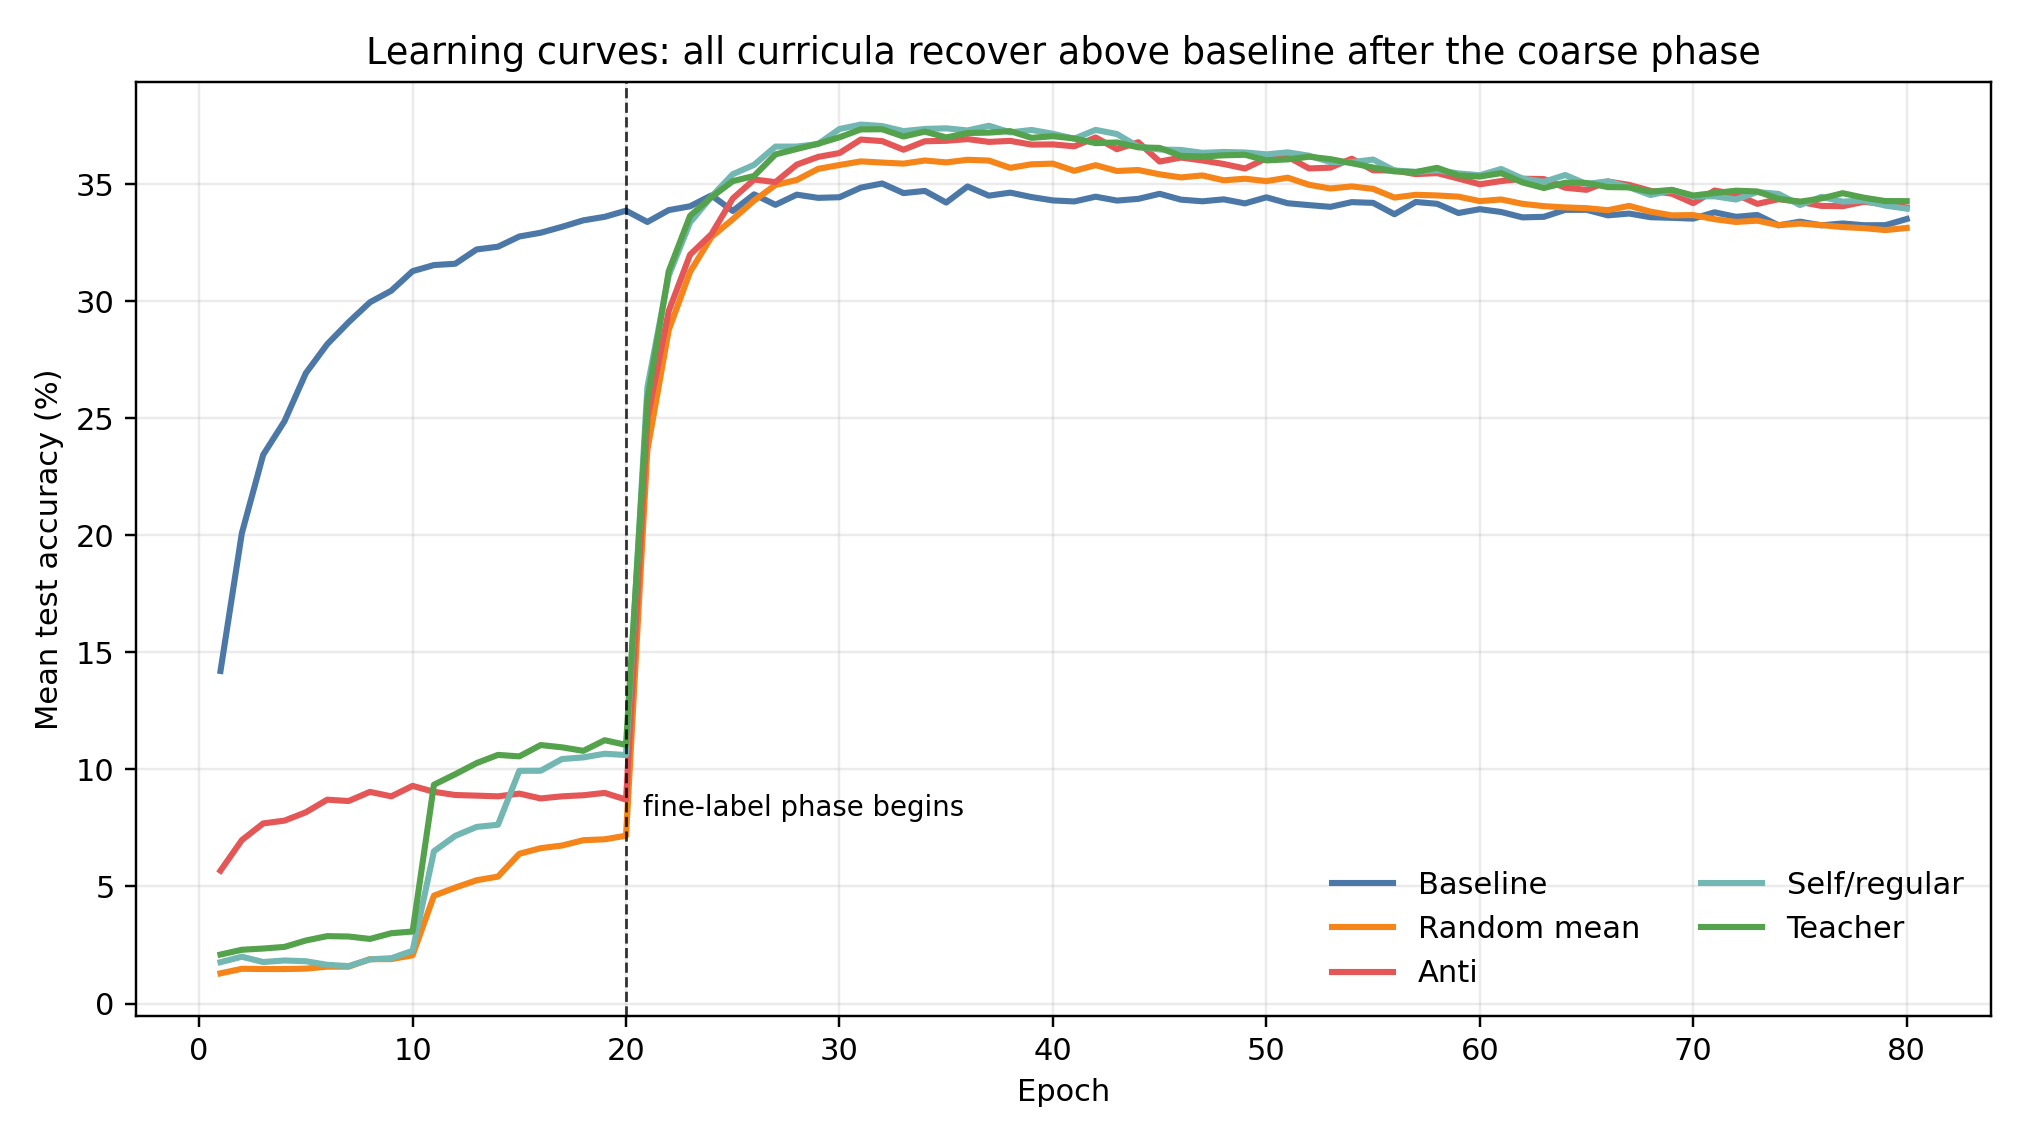
\includegraphics[width=0.92\textwidth]{figures/teacher_hierarchy_learning_curves_lr001.png}
    \caption{Mean test-accuracy trajectories. Random, anti, self, and teacher
    curricula all pay an early fine-label accuracy cost, but recover above the
    baseline region after the switch back to fine labels. Curves are means over
    seeds; random is averaged within seed first.}
    \label{fig:teacher-hierarchy-learning-curves}
\end{figure}

Figure~\ref{fig:teacher-hierarchy-switch-zoom} zooms into the switch region. At
epoch 20 the baseline is around 33.9\%, while the curriculum variants are far
lower: random is about 7.2\%, anti about 8.7\%, self about 10.6\%, and teacher
about 11.0\%. One epoch after the switch, the random and anti curves have already
jumped substantially, and by roughly epoch 30 the structured curricula are above
the baseline. This suggests that the coarse phase does not simply delay
learning; it changes the state from which fine-label training resumes.

\begin{figure}[h]
    \centering
    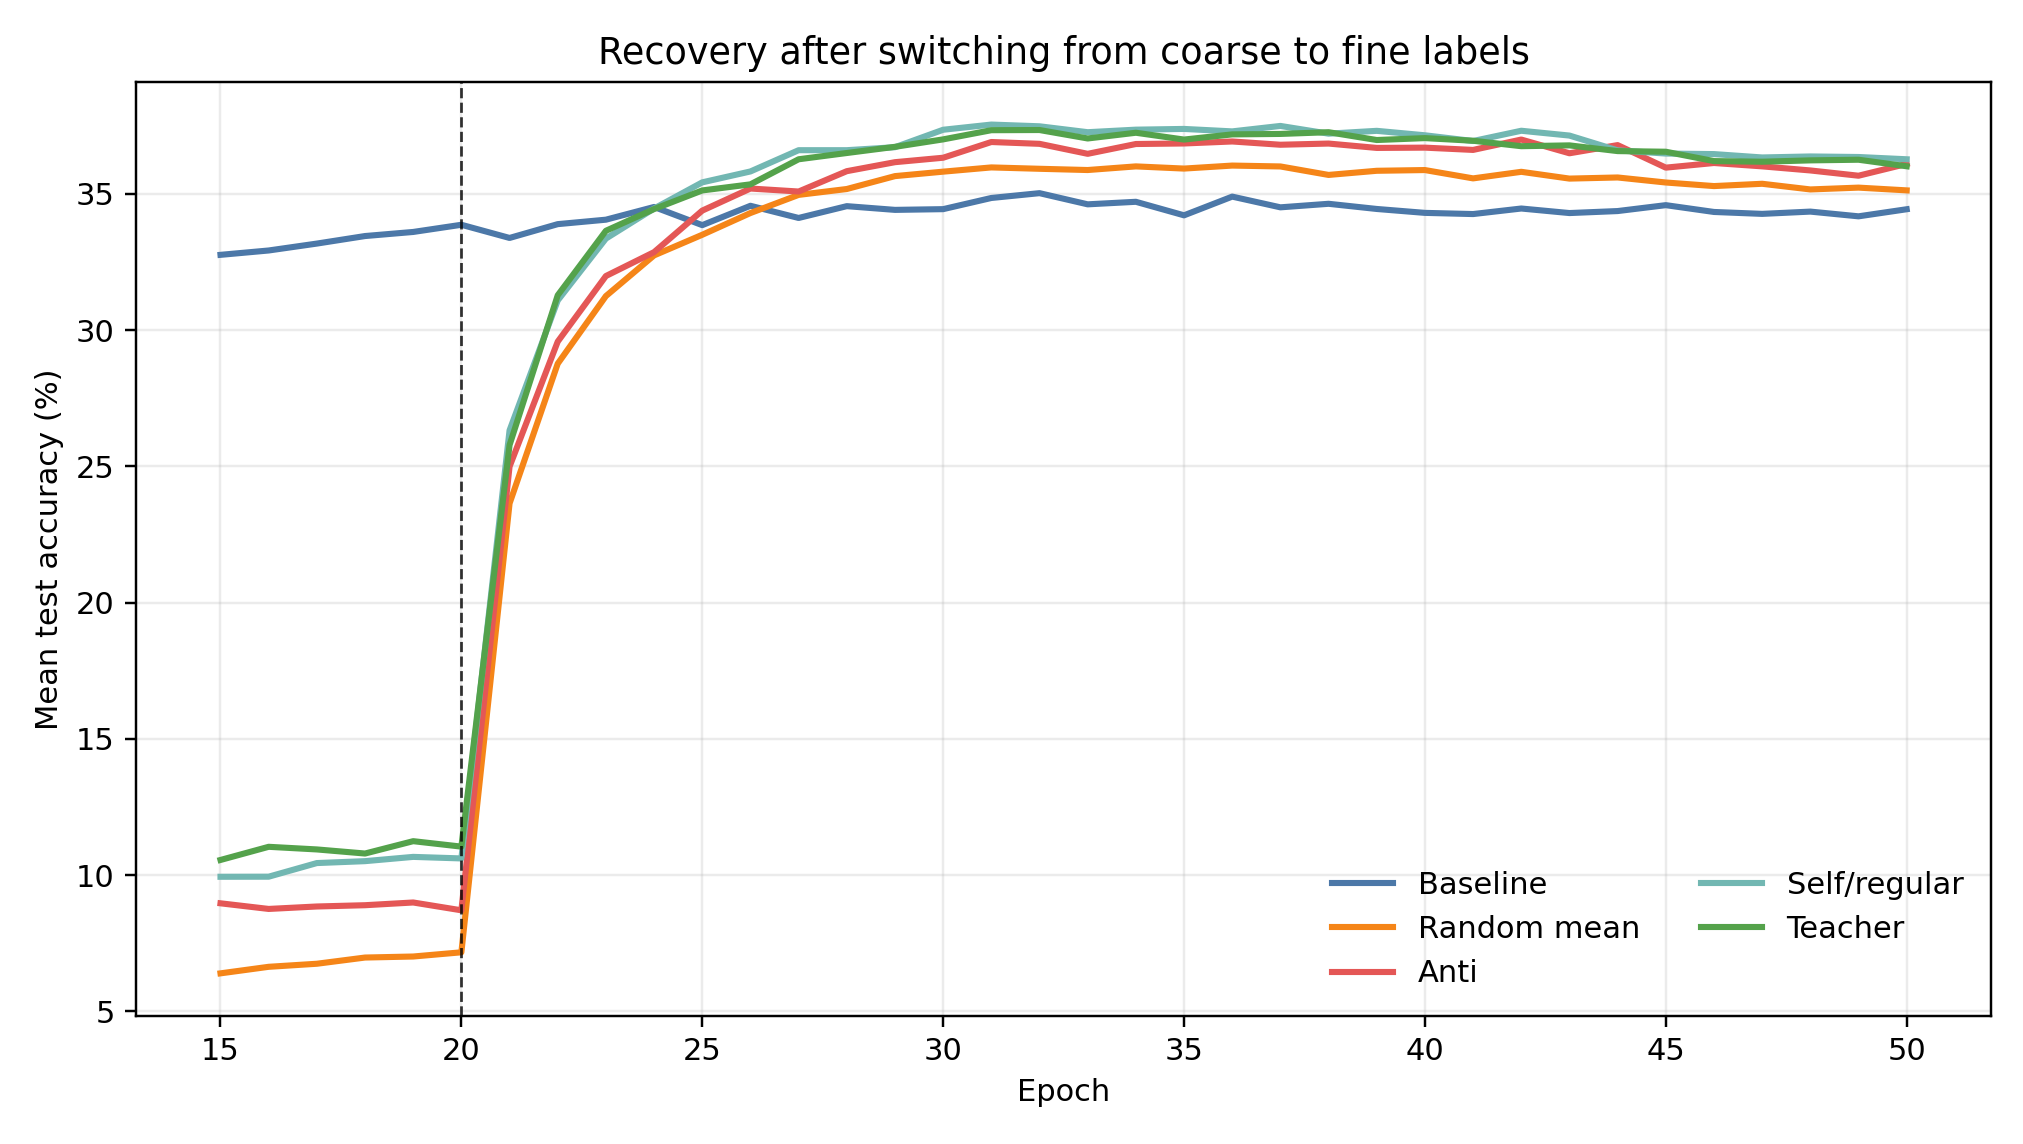
\includegraphics[width=0.92\textwidth]{figures/teacher_hierarchy_switch_zoom_lr001.png}
    \caption{Zoom around the transition from coarse labels to fine labels. The
    curricula are much worse on the fine-label metric during the coarse stage,
    but recover quickly after epoch 20.}
    \label{fig:teacher-hierarchy-switch-zoom}
\end{figure}

\section{Snapshot view}

Figure~\ref{fig:teacher-hierarchy-epoch-snapshots} summarizes the same dynamics
at selected epochs. It is useful because it separates three regimes. Before the
switch, the baseline dominates the fine-label metric. Immediately after the
switch, the curricula are still recovering. By epoch 30 to 50, the curriculum
runs are generally above the baseline. By epoch 80, the advantage is smaller,
which explains why final accuracy is less informative than best accuracy in this
experiment.

\begin{figure}[h]
    \centering
    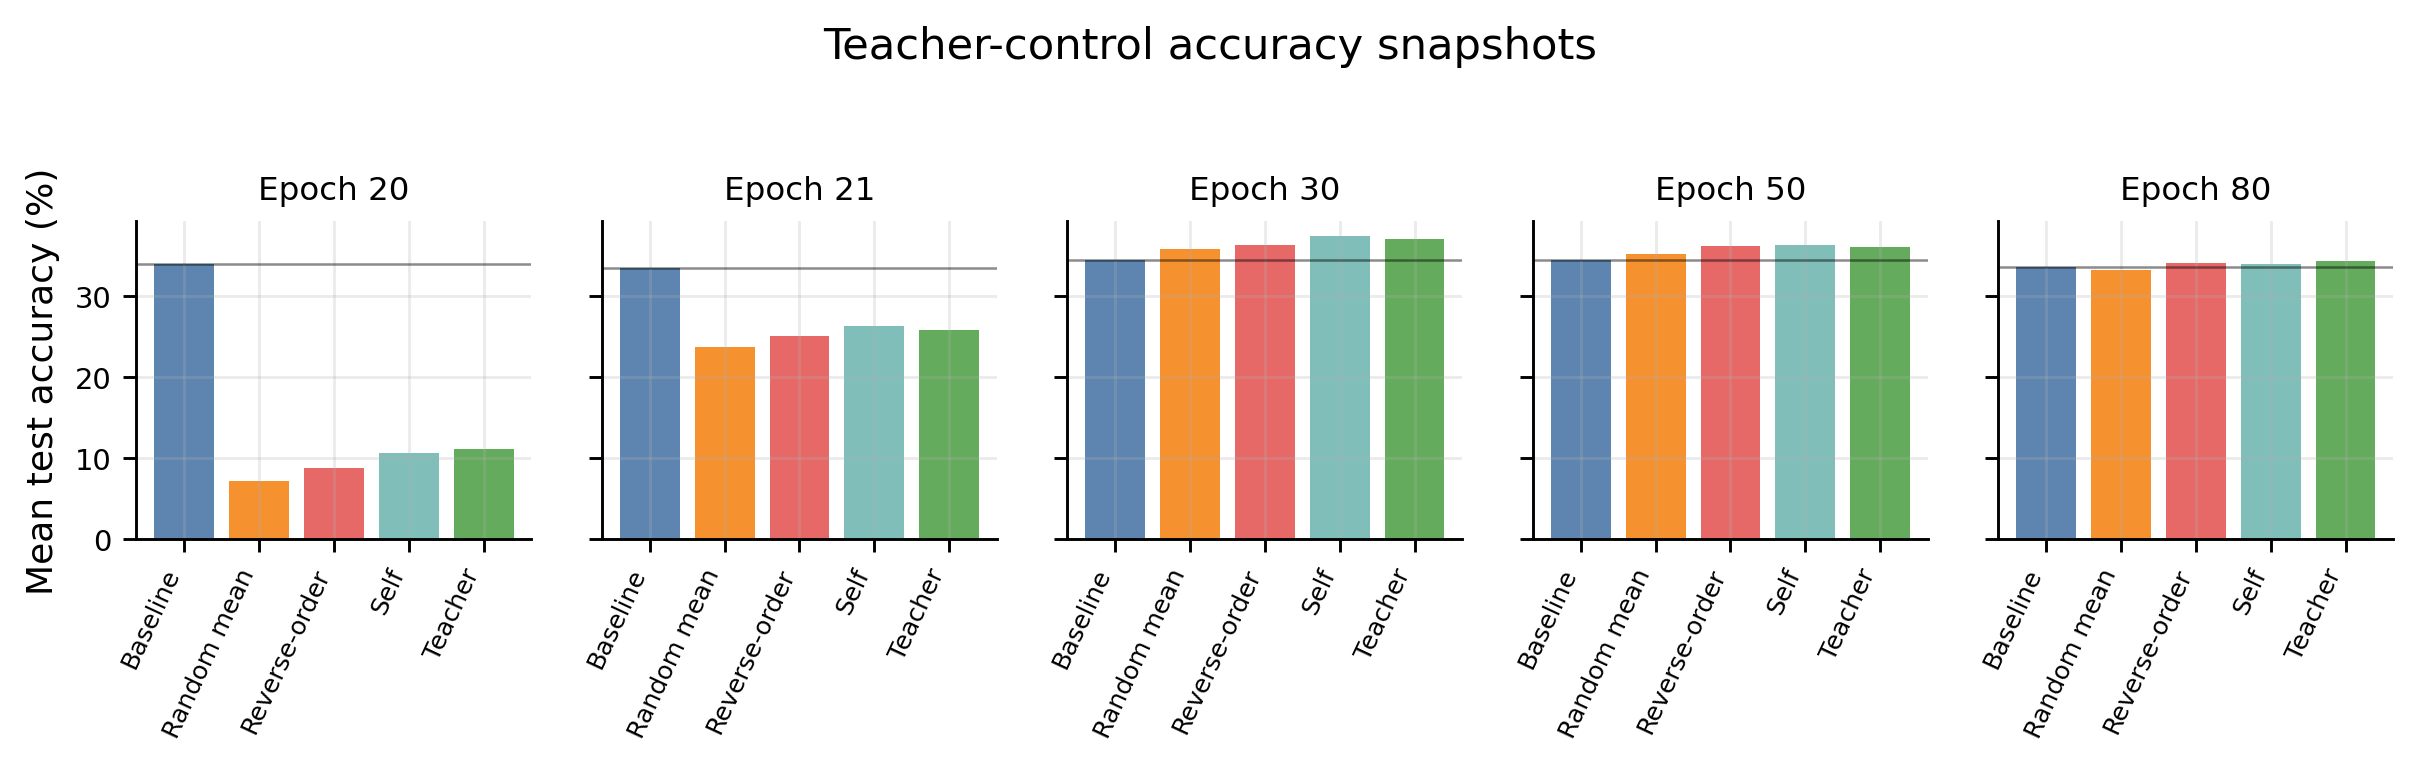
\includegraphics[width=0.98\textwidth]{figures/teacher_hierarchy_epoch_snapshots_lr001.png}
    \caption{Mean test accuracy at selected epochs. Random and anti-curriculum
    are below baseline during the coarse phase but above baseline after recovery.
    The structured self and teacher hierarchies remain the strongest peak-accuracy
    conditions on average.}
    \label{fig:teacher-hierarchy-epoch-snapshots}
\end{figure}

\section{Interpretation of random and anti-curriculum controls}

The random-control result is the most important caution for interpretation. If a
random hierarchy improves peak accuracy by nearly one percentage point, then a
positive curriculum result is not automatically evidence that the hierarchy is
semantically meaningful. The curriculum procedure itself has an effect. In this
implementation, that effect likely combines several mechanisms: fewer effective
decision regions in the first stage, a different early representation-learning
path, reduced pressure to separate all fine classes immediately, and a form of
regularization similar in spirit to imposing a temporary output bottleneck.

At the same time, the random result does not erase the role of structure. The
self and teacher hierarchies are still about 1.3--1.4 percentage points above
the random mean. Moreover, the random condition was a strong control because it
preserved the hierarchy shape and cluster sizes. The only thing destroyed was
which CIFAR-100 classes were grouped together. The remaining gap therefore
supports the claim that class grouping matters, even though it is not the only
source of the gain.

The anti-curriculum is also informative. It is closer to the structured methods
than to the random mean in peak accuracy, despite using the wrong temporal order.
This means that reversed curricula should not be interpreted as pure negative
controls. They still expose the student to structured class bundles and can still
induce useful representations. The corrected teacher anti-curriculum reached a
+2.06 point best-accuracy gain, lower than self and teacher but clearly above
random. The easy-to-hard direction therefore helps, but the grouping information
itself appears more important than the temporal order in this particular fixed
20-epoch schedule.

Finally, the teacher hierarchy did not decisively beat the self-derived hierarchy
in peak accuracy. The corrected teacher reached a much stronger operating point
than the first bootstrap teacher, but its student curriculum obtained 37.69\%
best accuracy, essentially tied with the self hierarchy at 37.76\%. The teacher
hierarchy did improve trajectory/AUC relative to self and random, but the peak
result suggests that hierarchy quality alone is not the only bottleneck. The
fixed schedule, the output-space marginalization objective, and the weak CNN
student capacity all likely constrain the achievable benefit.

\section{Updated conclusion}

The teacher probe and follow-up controls support a more nuanced conclusion than
"better hierarchy solves curriculum learning." A strong transfer teacher can be
trained cheaply and produces a plausible hierarchy. That hierarchy clearly beats
random grouping, and meaningful structure improves over arbitrary coarsening.
However, arbitrary coarsening itself is beneficial in this CIFAR-100
\texttt{cnn\_w0.5} setting, and even the anti-curriculum remains above baseline.
The evidence therefore separates two effects: a general coarse-label warm-up or
regularization effect, and an additional hierarchy-structure effect.

For the thesis, the strongest defensible statement is that hierarchy quality
matters, but it is not the only reason coarse-to-fine curricula help. Random and
anti-curriculum controls reveal that output-space coarsening can improve peak
accuracy even when the grouping is weak or the temporal order is wrong. Structured
self-derived and teacher-derived hierarchies improve further, but the corrected
teacher hierarchy does not robustly dominate the self-derived hierarchy in peak
accuracy. This finding should be moved into the main discussion because it
clarifies why positive curriculum gains must be interpreted against both random
and anti-curriculum controls.
